\documentclass[10.9pt]{article}
\usepackage[utf8]{inputenc}
\usepackage[parfill]{parskip}
\usepackage{graphicx}
\usepackage{amsmath}
\usepackage[title]{appendix}
\usepackage[margin=0.7in]{geometry}
\usepackage{amsmath,graphicx,psfrag,pstricks}
\def\n{\noindent}
\def\u{\underline}
\usepackage{gensymb}
\def\hs{\hspace}
\newcommand{\thrfor}{.^{\displaystyle .} .}
\newcommand{\bvec}[1]{{\bf #1}}
\usepackage{graphicx}
\usepackage{rotating}
\graphicspath{{Plots/}}
\usepackage{amsmath}
\usepackage{booktabs}
\usepackage{siunitx}
\usepackage{amssymb}
\usepackage[utf8]{inputenc}
\usepackage[justification=centering]{caption}
\usepackage{float}
\usepackage{listings}
\usepackage{color} %red, green, blue, yellow, cyan, magenta, black, white
\definecolor{mygreen}{RGB}{28,172,0} % color values Red, Green, Blue
\definecolor{mylilas}{RGB}{170,55,241}
\lstset{language=Matlab,%
    %basicstyle=\color{red},
    breaklines=true,%
    morekeywords={matlab2tikz},
    keywordstyle=\color{blue},%
    morekeywords=[2]{1}, keywordstyle=[2]{\color{black}},
    identifierstyle=\color{black},%
    stringstyle=\color{mylilas},
    commentstyle=\color{mygreen},%
    showstringspaces=false,%without this there will be a symbol in the places where there is a space
    numbers=left,%
    numberstyle={\tiny \color{black}},% size of the numbers
    numbersep=9pt, % this defines how far the numbers are from the text
    emph=[1]{for,end,break},emphstyle=[1]\color{red}, %some words to emphasise
    %emph=[2]{word1,word2}, emphstyle=[2]{style},  
}
\title{Part IIA Project - SF1: Data Analysis - First Interim Report}
\author{Bailey Brookes | Corpus Christi | bdb31}
\date{\today}

\begin{document}
\maketitle

\section{DFT vs FFT}
While the DFT is fairly simple to compute, it has redundancy in it which causes it to be slow. It calculates the same exponential base (weights) numerous times. The FFT uses this recursion and redundancy to speed up the process. While the DFT requires $2N + 2N$ operations to calculate each point $X_p$ and $X_{p+\frac{N}{2}}$, giving it complexity $O(N^2)$, the FFT has $2N + 2+2$ operations, meaning it has complexity $O(N\log_2N)$. Figure \ref{DFTvFFT} shows how the reduction in complexity results in a much faster computing time for longer data length.

\section{Effects on the FFT}
\subsection{Data Length}
FFT resolution increases with data length $N$ and there are more frequency bins meaning a smaller frequency difference between bins. This increase in sharpness in shown in Figure \ref{Length}. This is why signals are sometimes 'zero padded'. Adding zeros to the end of the signal achieves two things:
\begin{enumerate}
	\item By adding enough zeros to make the data length a power of two, the FFT becomes much more efficient.
	\item The greater the length of data, the higher the resolution.
\end{enumerate}
Zero padding also does not change the frequency content of the signal, making this technique extremely useful.

\subsection{Windowing}
Windowing reduced the effect of spectral leakage caused by the sharp cut off caused by finite sampling. Figure \ref{Window_compare} shows this leakage for a rectangular (unwindowed) sinewave as well as a hann, hamming and triangle window. Windowing reduces the signal to zero at the end of the sampling times so there is no sharp frequency change when the sample is repeated in order to compute the FFT. Sharp charges in time result in broad frequency spectrum. This, as well as the true signal being spilt across multiple frequency bins if the frequency of the signal does not perfectly fit into one bin, is the spectral leakage.
\subsection{Noise}
The addition of Gaussian noise to the pure tone decreases the relative size of the spectral peak with respect to the surrounding noise. This is because white noise, such as Gaussian white noise, is flat across all frequencies, meaning the base level is higher for more and more noise making the size of the peak for the tone relatively smaller, as shown in Figure \ref{Noise}.

\subsection{Amplitude Modulation}
Figure \ref{Modulation} shows the effect 3 different modulation schemes have on a pure tones fft.

Random noise modulation has a similar effect to the additive Gaussian noise from before, decreasing the relative size of the main spectral peak dramatically.

Linear increase modulation  causes a large increase in spectral leakage. This is due to to effects of windowing,as described above. The sharp change from a high amplitude back to zero when the signal is repeated has a broad frequency spectrum, resulting in this large leakage. This is similar to the effects of using a rectangular window.

The periodic  modulation similar to that used in amplitude modulation (AM) for radio, resulting in peaks at both the tones frequency (in this case, the higher frequency 'carrier') and peaks either side which are the upper and lower side-band frequencies. The spacing between them is the modulation frequency itself of 0.01Hz.
\section{FFT on Real Data}
\subsection{FFT on Music}
The file piano\_clean.wav was loaded into Matlab and an attempt made to isolate its six notes in the spectrum. This was done by 'eyeballing' the location of the notes, windowing each note with a hann window, which gave the sharpest roll off in frequency as found out before. Results from this are shown in Figure \ref{Piano}, which can be compared to the full frequency spectrum in Figure \ref{Piano_OG}. 

The sound file has a scale of increasing pitch which is clearly seen in Notes 4 through 6. Note 1 shows the longer held note and has clearly defined peaks. Three peaks suggest a chord is being played.
\subsection{FFT on Speech}
The file f1lcapae.wav  was loaded into Matlab and an attempt made to isolate individual syllables of the first phrase. This is much harder due to the more 'continuous' nature of speech, rather than the clear separate notes in the piano file. Figure \ref{Speech}  shows the full spectrum and attempts to isolate individual syllables, again using a hann window to window to syllable of interest.

Sounds 4 and 6 are sharp 't' sounds and have a broad spectrum while 2 is an 'o' and 7 a 'y' sound which have quite peaky spectrum, suggesting vowels have sharper peaks in there spectrum and consonants a more broader spectrum.


\subsubsection{Challenge Question: Organ.wav}
Organ.wav was loaded into Matlab and its first channel windowed with a hann window and then zero padded with $1 \times 10^6$ zeros to produce the frequency spectrum in Figure \ref{Organ_fft}. The sound file is messy with many notes merged into one, as can be seen in the time domain plot of the organ in Figure \ref{Organ_time} and in the large number of peaks in the frequency spectrum. By measuring the frequency at which these peaks occur and comparing them to the frequencies of musical notes (such as the table of them from \underline{https://pages.mtu.edu/~suits/notefreqs.html}) the musical notes present can be extracted.Taking 'Middle $C$ as $C_4$ and $A$ at 440Hz, a few examples are:

\begin{itemize}
\item Main peak at 468.4Hz, corresponding to $A_3^\#$
\item Peak at 156.8, corresponding to $D_3^\#$
\item Peak at 627.4, corresponding to $D_4^\#$, and an octave higher than the previous note.
\end{itemize}

Overall there are 10 large peaks suggesting louder notes with several small peaks suggesting other quieter notes, such as sustained notes from before the recording was taken, are present.

\appendix
\section{Plots}

\begin{figure} [H]
\centering	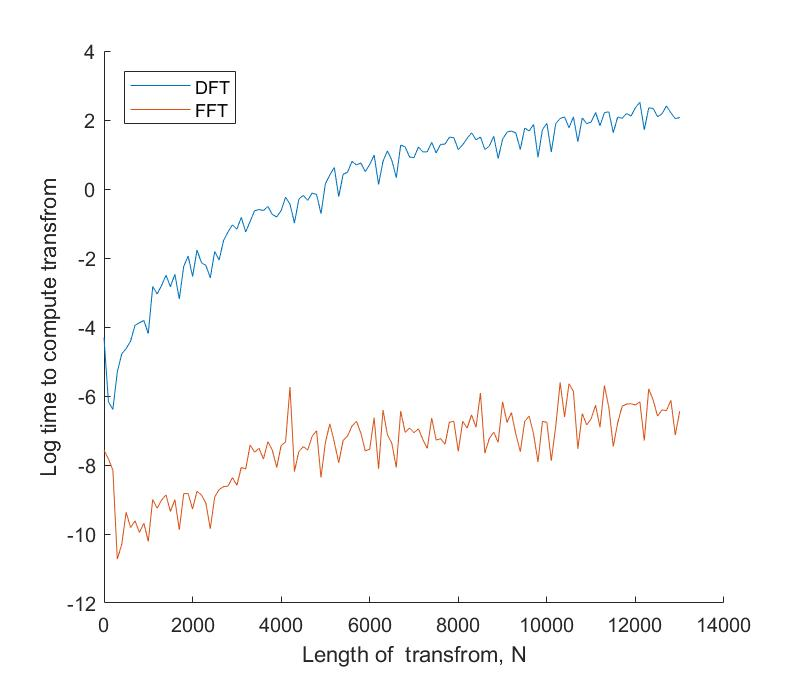
\includegraphics[scale = 0.4]
{DFTvFFT}
\caption{Comparison of the speed of the DFT and FFT, measured by the log of the time taken to compute with N samples. It is clear to see the DFT is slower and getting slower much faster than the FFT}
\label{DFTvFFT}
\end{figure}

\begin{figure} [H]
\centering	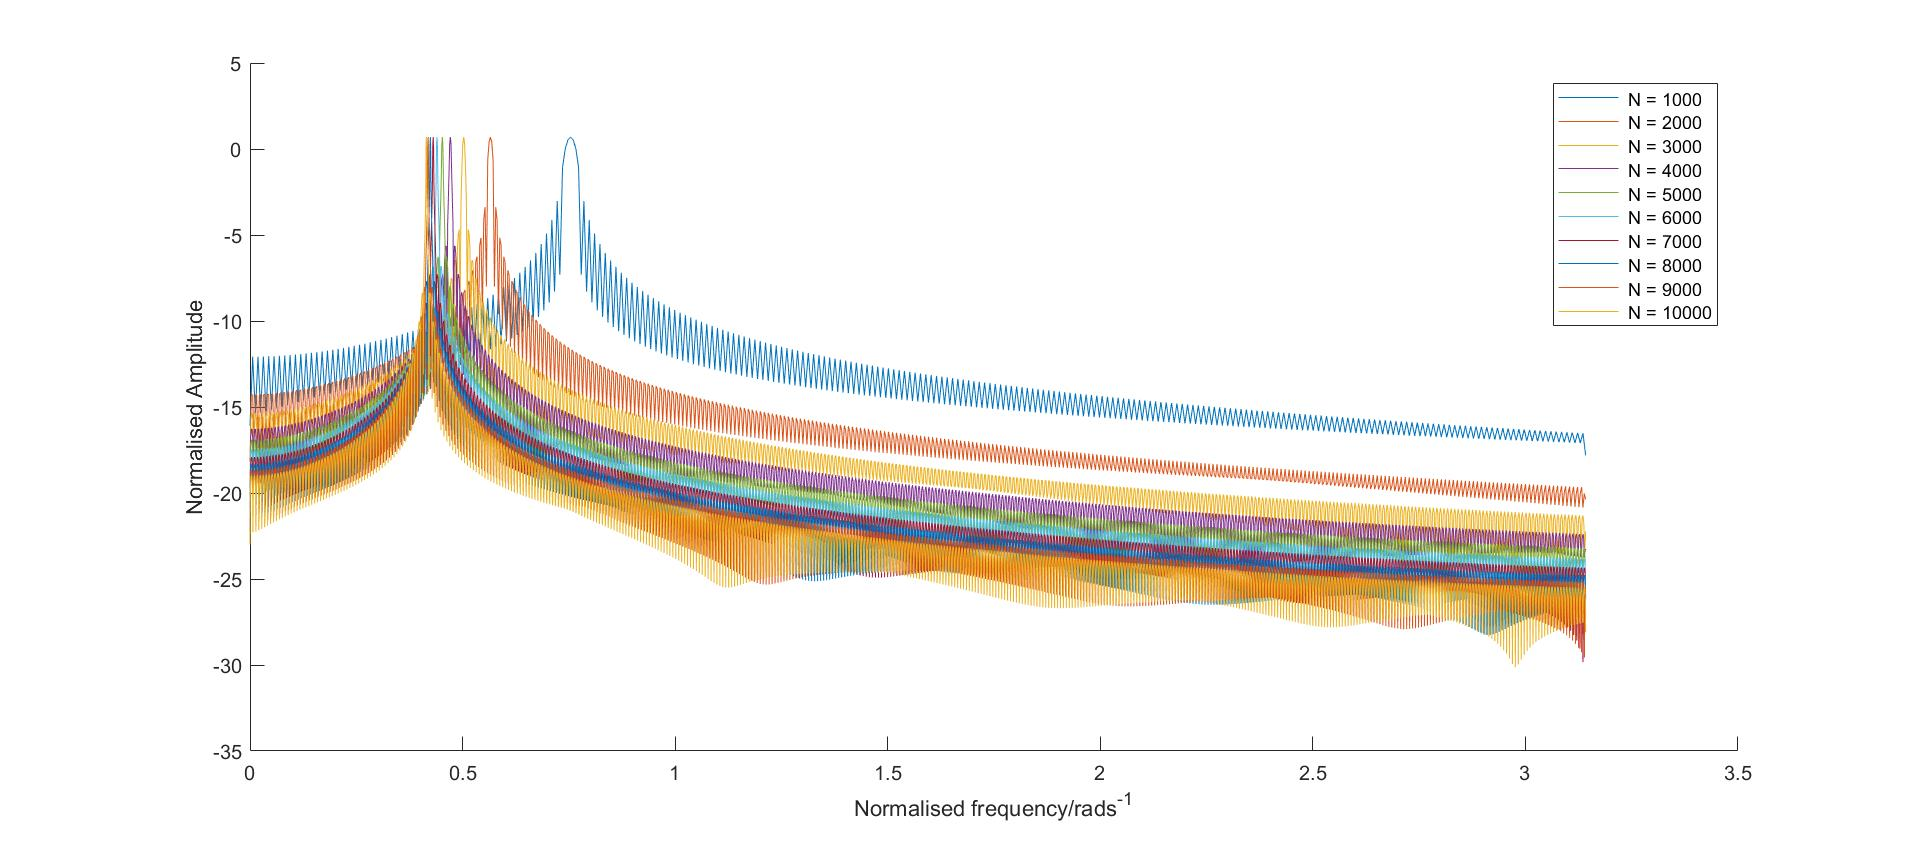
\includegraphics[scale = 0.3]
{Length}
\caption{Log spectral magnitude plots for different lengths of FFT.}
\label{Length}
\end{figure}

\begin{figure} [H]
\centering	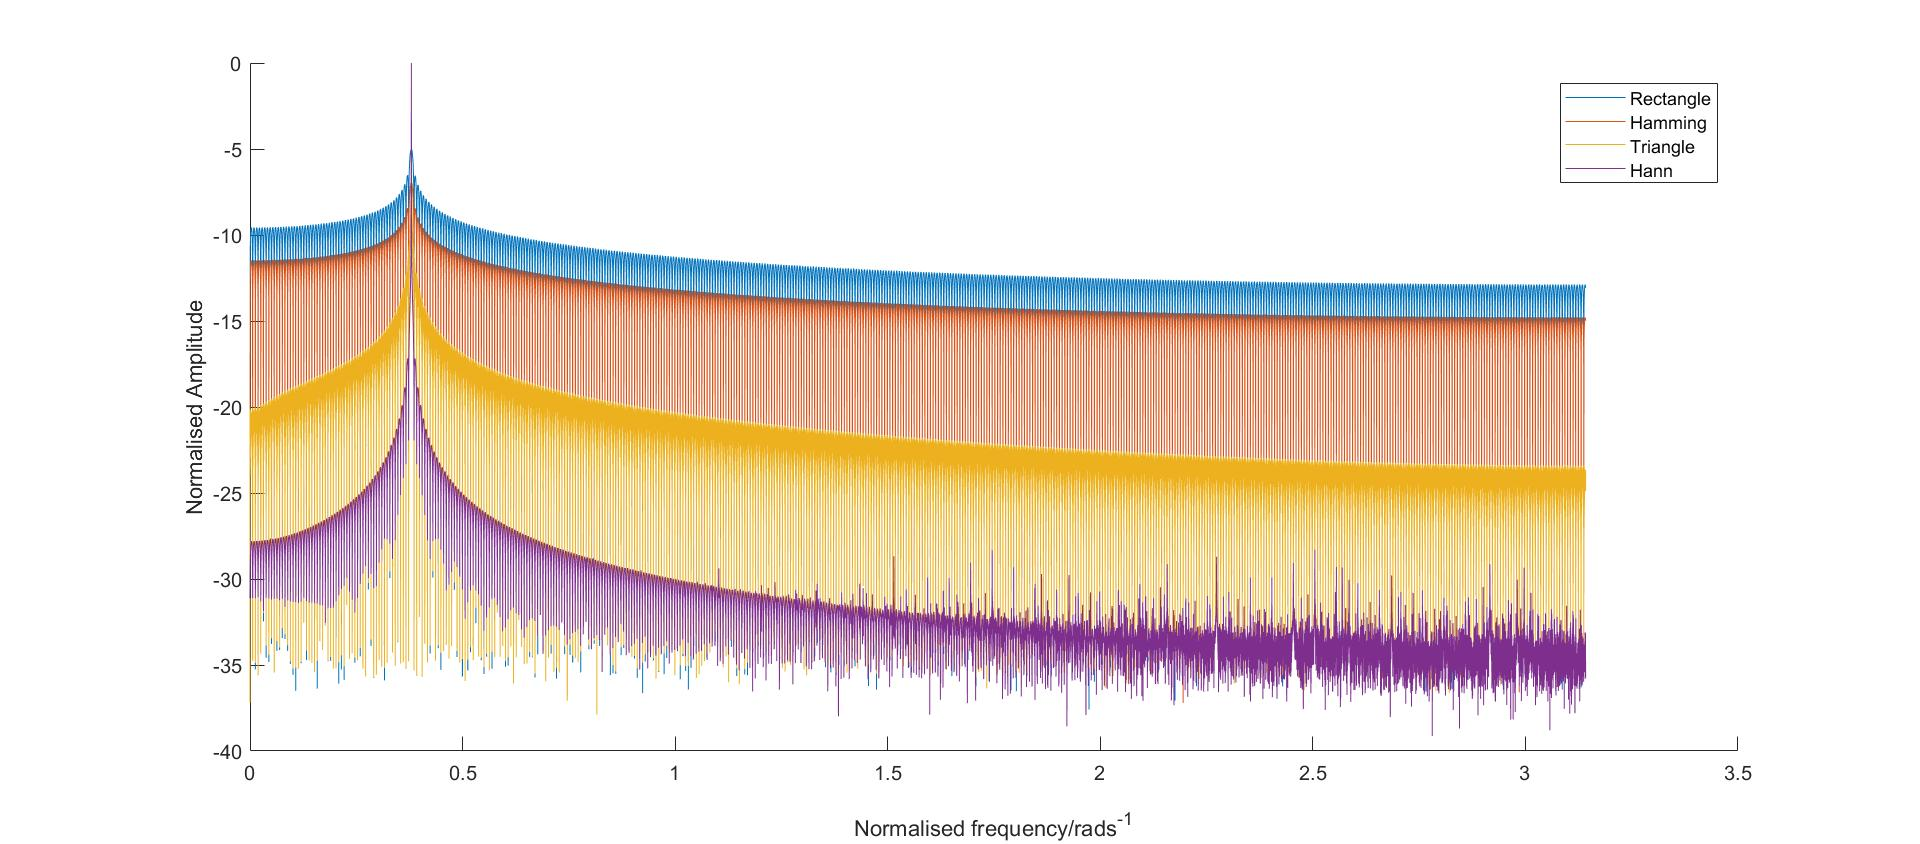
\includegraphics[scale = 0.3]
{Window_compare}
\caption{Log spectral magnitude plots for different lengths of FFT.}
\label{Window_compare}
\end{figure}

\begin{figure} [H]
\centering	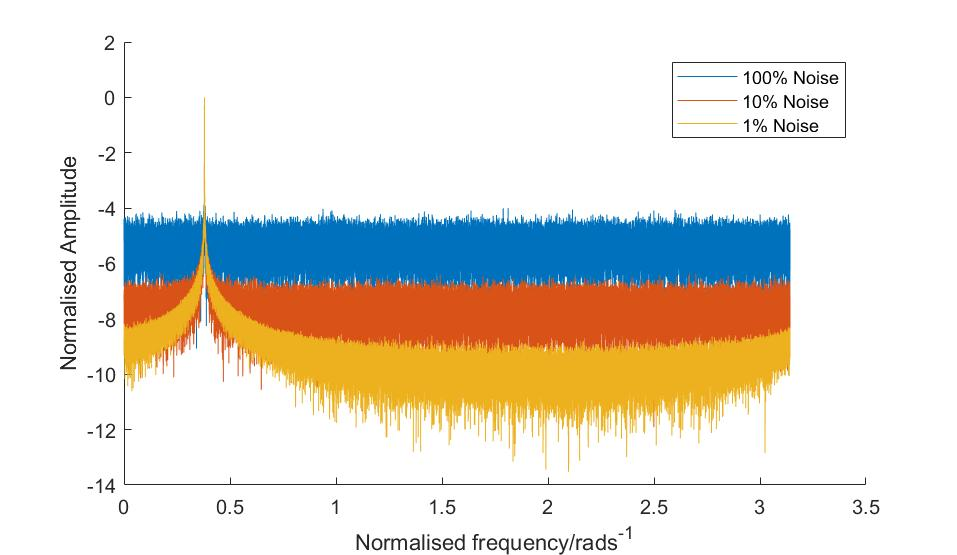
\includegraphics[scale = 0.4]
{Noise}
\caption{Normalised Log spectral magnitude plots for different windows on a pure sine tone}
\label{Noise}
\end{figure}

\begin{figure} [H]
\centering	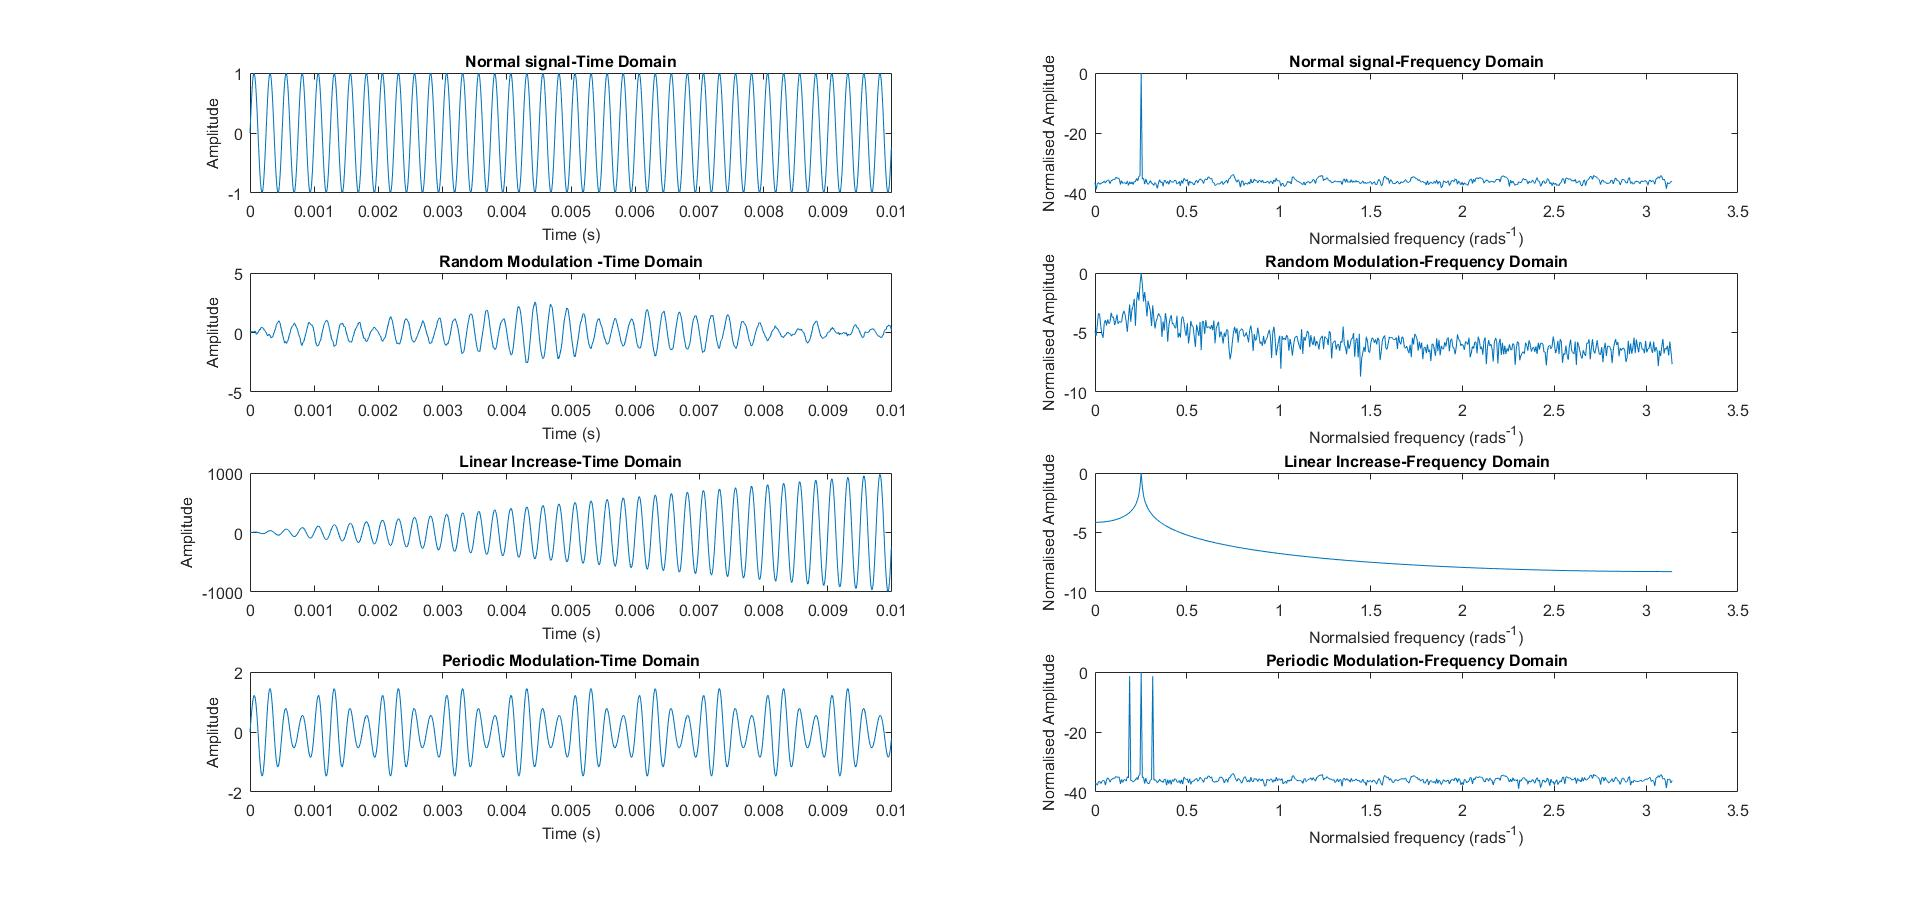
\includegraphics[scale = 0.28]
{Modulation}
\caption{Effect different modulation schemes have on the spectral content}
\label{Modulation}
\end{figure}

\begin{figure} [H]
\centering	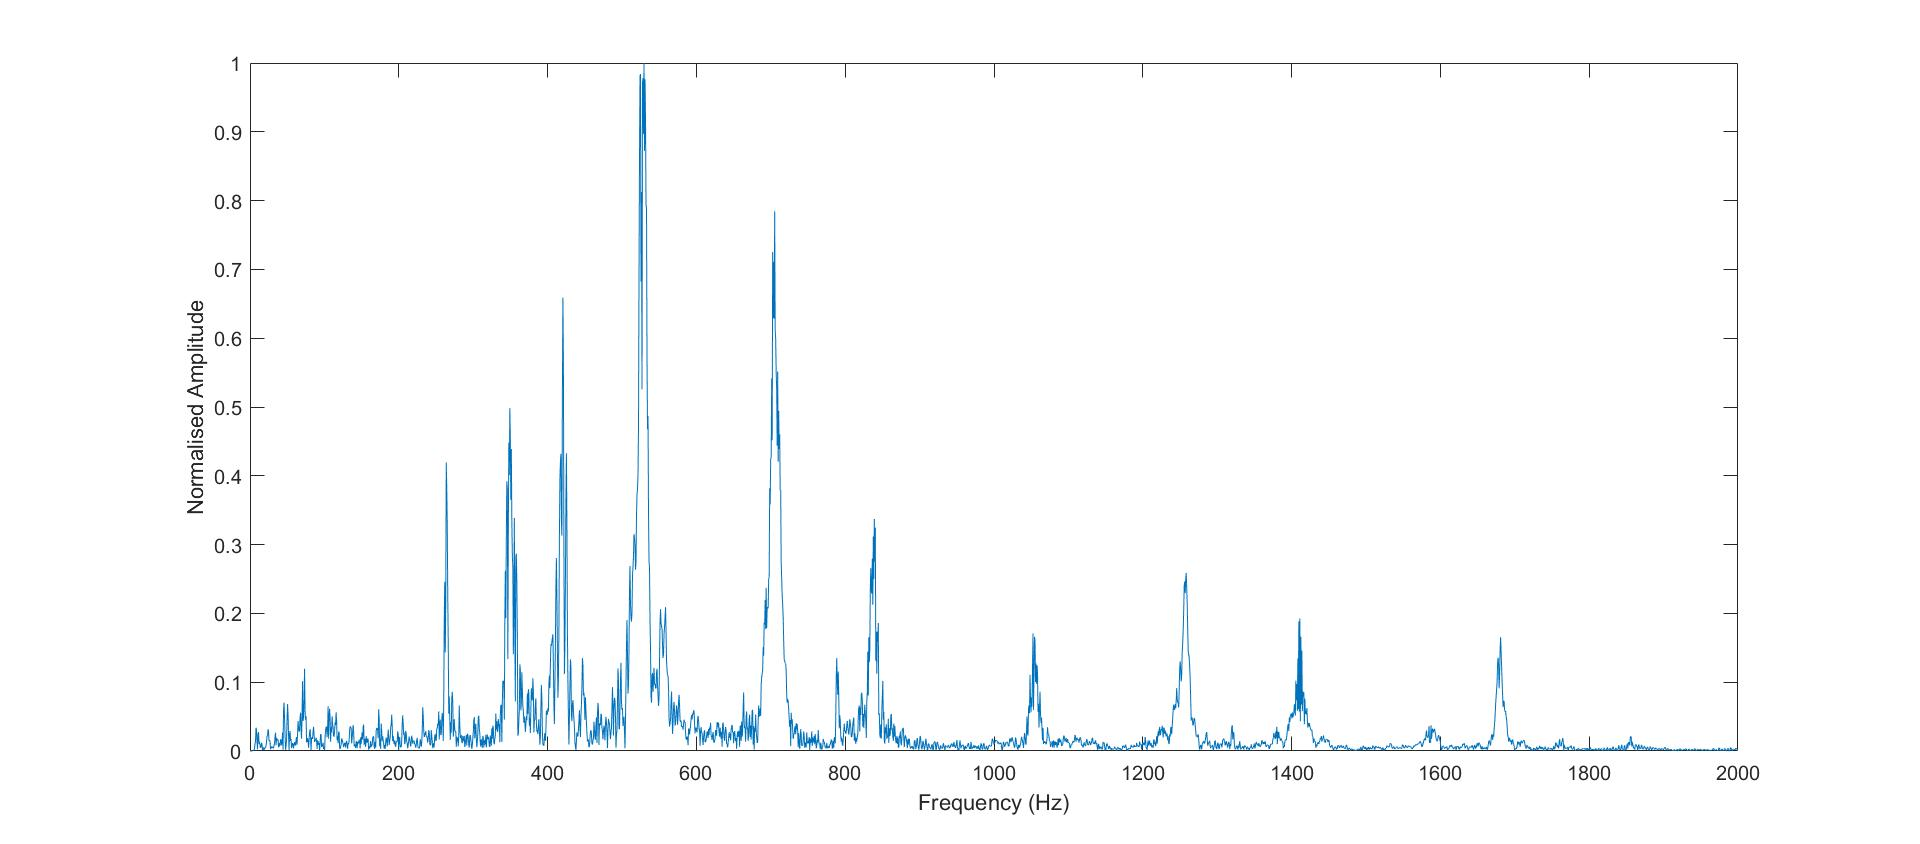
\includegraphics[scale = 0.2]
{Piano_OG}
\caption{Spectrum of piano\_clean.wav}
\label{Piano_OG}
\end{figure}

\begin{figure} [H]
\centering	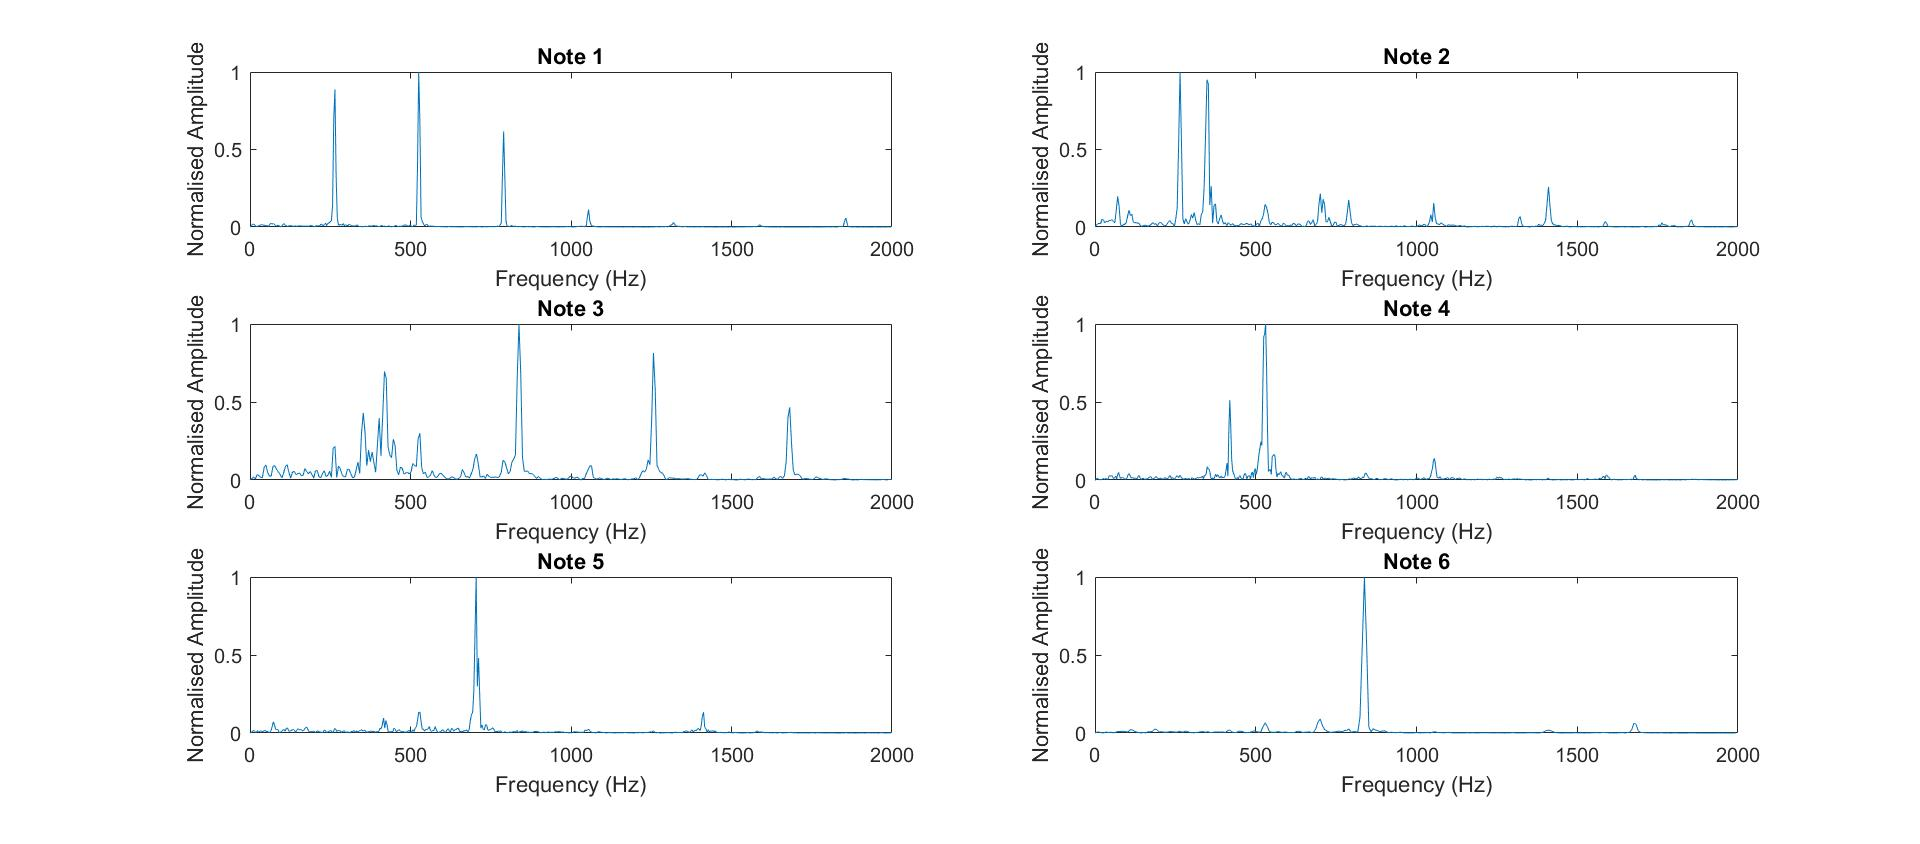
\includegraphics[scale = 0.3]
{Piano}
\caption{Spectrum's of piano\_clean.wav individual notes}
\label{Piano}
\end{figure}

\begin{figure} [H]
\centering	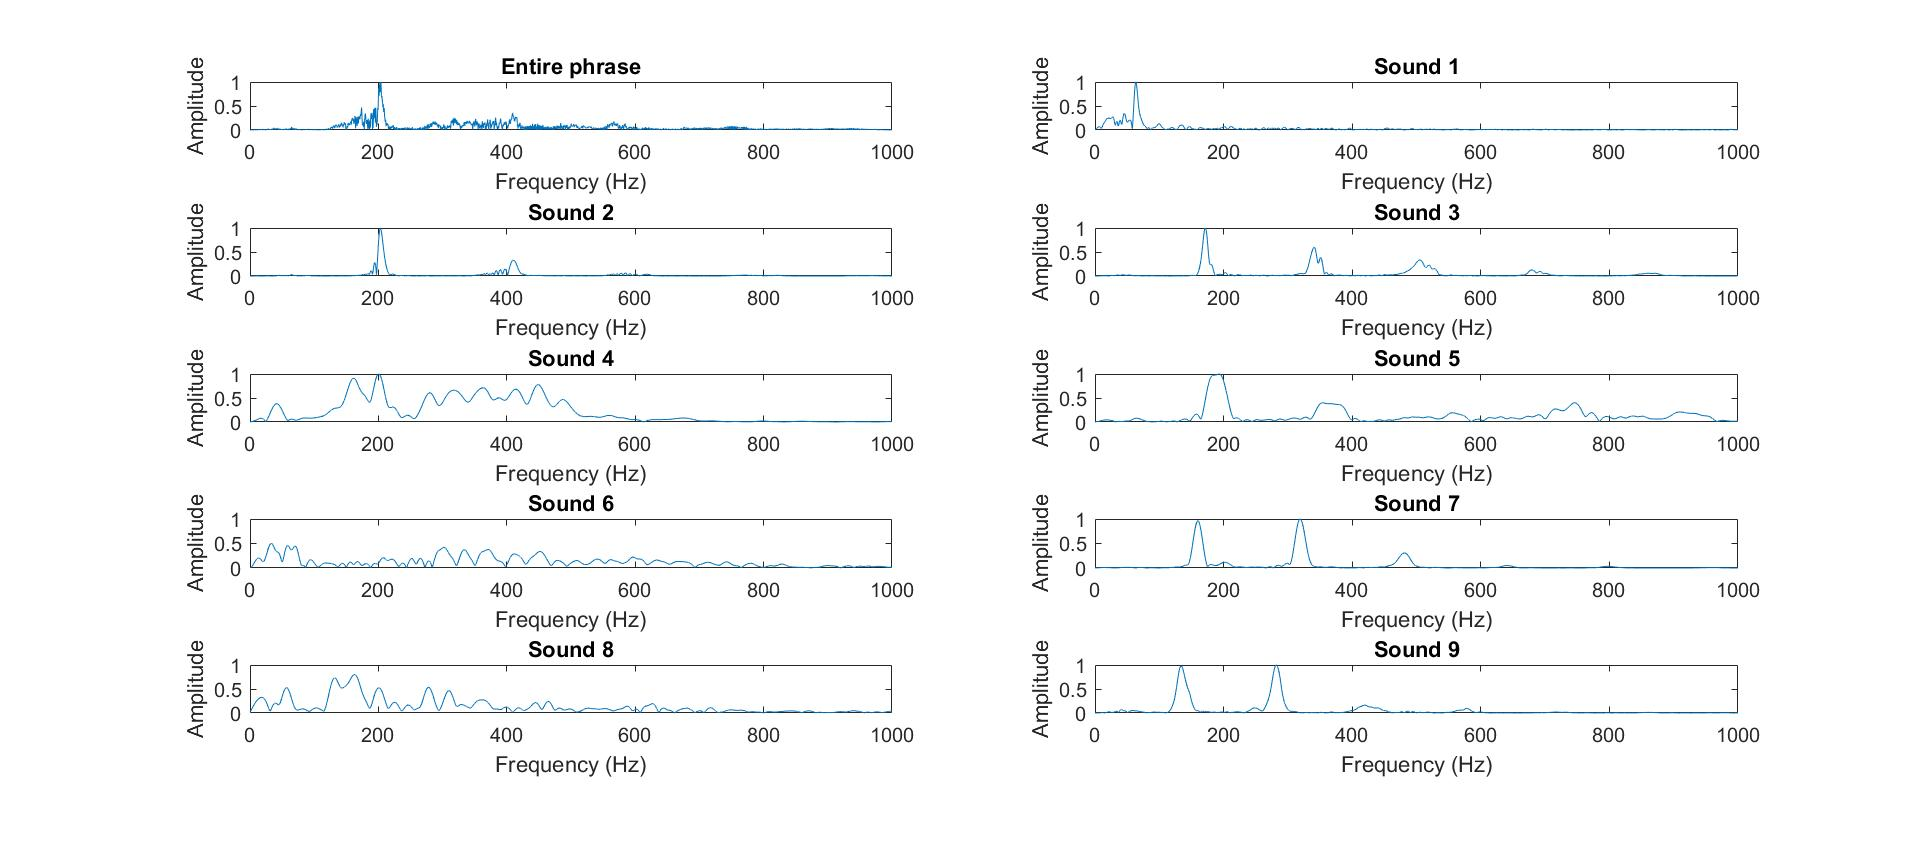
\includegraphics[scale = 0.3]
{Speech}
\caption{Spectrum's of f1lcapae.wav}
\label{Speech}
\end{figure}

\begin{figure} [H]
\centering	\includegraphics[scale = 0.3]
{Organ_time}
\caption{Time domain plot of organ.wav}
\label{Organ_time}
\end{figure}

\begin{figure} [H]
\centering	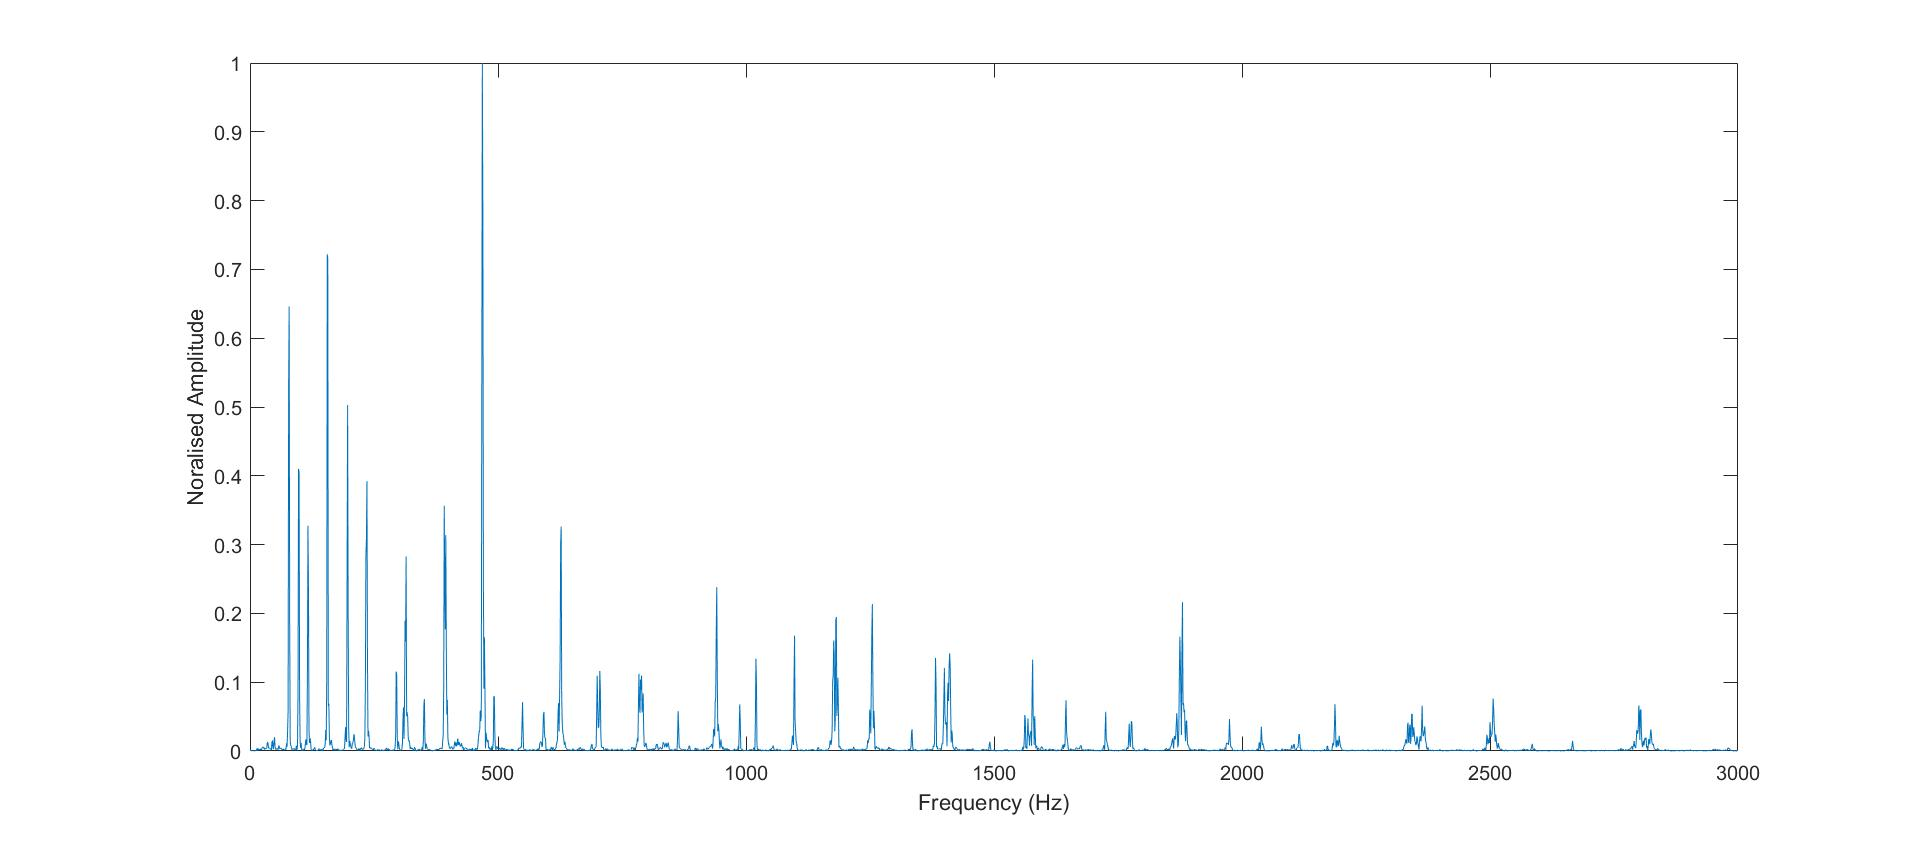
\includegraphics[scale = 0.3]
{Organ_fft}
\caption{Spectrum's of organ.wav}
\label{Organ_fft}
\end{figure}


\end{document}